%!TEX root = ../main.tex

\section{Mean-variance optimization}
\label{sec:mean_variance}

The issue of how a factor portfolio should be allocated is highly relevant to portfolio managers. Common strategies include equal weights and mean-variance optimization. Based on abnormal return regressions and the work on mean-variance portfolios in \textcite{HubermanKandel1987}, \textcite{FF2015} conjecture that the HML factor will not improve the mean-variance tangency portfolio when added to a portfolio of Mkt-RF, SMB, RMW and CMA. Differently put, this is equivalent to HML having a zero weight in mean-variance optimization. Subject to a constraint of no negative weights, this section will examine what the mean-variance weights are, given different asset universes.

We consider mean-variance optimization based on full-sample estimates of the means and covariance matrices of the six factors, as well as in a dynamic setting based on the conditional distributions of returns implied by our copula model. We consider portfolios with and without momentum (five- and six-factor portfolios, respectively) and how portfolio weights change when replacing HML with CMA and vice versa.

% \subsection{Implementation}

% In mean-variance investing, it becomes important to distinguish what we mean by investing in a zero-cost portfolio. While investing in a zero-cost portfolio does per se not require any cash upfront, brokers and the Federal Reserve's Regulation T require collateral for short positions, and when buying on margin.\footnote{U.S. Government Publishing Office. (2016). \textit{Regulation T: Credit by Brokers and Dealers}. Available from: \url{http://www.ecfr.gov/cgi-bin/text-idx?c=ecfr&sid=635f26c4af3e2fe4327fd25ef4cb5638&tpl=/ecfrbrowse/Title12/12cfr220_main_02.tpl}} It is therefore not the case that an investor may earn the factor strategy premia without investing some upfront capital. The degree of leverage chosen will impact the cash required upfront, as well as determine the risk that the portfolio receives a margin call, in which additional collateral must be posted to keep the positions. While this is an interesting matter and discussion in its own right, this thesis will analyze factor returns only as excess returns on zero-cost portfolios, without concerning the costs of implementation. While this is a simplification, it is not quite as strong as it seems for the purpose at hand. As we are not concerned with the absolute performance of strategies, but instead with the optimized weights over time, the transaction costs are not relevant, as long as all factors have similar transaction costs.

% We run mean-variance optimizations in both the five- and six-factor models, and in both cases consider the effects of including and excluding HML and CMA one at a time.

% \begin{table}[!htbp] \centering 
%   \caption{Asset universes} 
%   \label{fig:asset_universes} 
% \begin{tabularx}{\textwidth}{X}
% \\[-1.8ex]\toprule
% \\[-1.8ex] 
% \footnotesize The six asset universes considered in mean-variance investing
% \end{tabularx}
% \begin{tabularx}{\textwidth}{@{\extracolsep{0pt}}l c c c c c c } 
% \\[-1.8ex]\midrule 
%  Five-factor model 				& Mkt-RF & SMB & HML & CMA & RMW &	 	\\
%  Five-factor model (excl. HML) 	& Mkt-RF & SMB & 	 & CMA & RMW &	 	\\
%  Five-factor model (excl. CMA) 	& Mkt-RF & SMB & HML & 	   & RMW &	 	\\
%  \hline
%  Six-factor model 				& Mkt-RF & SMB & HML & CMA & RMW &	Mom 	\\
%  Six-factor model (excl. HML) 	& Mkt-RF & SMB & 	 & CMA & RMW &	Mom 	\\
%  Six-factor model (excl. CMA) 	& Mkt-RF & SMB & HML & 	   & RMW &	Mom 	\\
% \bottomrule \\[-1.8ex] 
% \end{tabularx} 
% \end{table}

\subsection{Optimization problem with restrictions}

Each week, we optimize for the maximum Sharpe ratio of a portfolio invested across factors. We impose two restrictions on our optimization problem. First, all factor weights must be positive. This reduces the problem with extreme weights, seen in the unconstrained optimization problem, and reflects a view that an investor will not bet against factors that have generated a history of positive premia. Second, factor weights must sum to unity, i.e. fully invested across factors. Together, these restrictions make the optimized weights more comparable to an equal-weights strategy and reflect the tangency weights subject to a constraint of no negative weights.

% Following \textcite{ChristoffersenLanglois2013}, we impose two general restrictions on the portfolios: First, all factor weights must be positive, as the interpretation of a negative factor weight is the same as betting against a factor that has been shown to generate a history of return premia. In addition, this resolves the issue of extreme weights, a common issue in unconstrained portfolios. Second, factor weights must sum to 1, as we do not consider the case of levered portfolios. This second restriction deviates slightly from \textcite{ChristoffersenLanglois2013}, who allow some leverage to the total portfolio in their maximum CRRA utility exercise. Given these two restrictions, our mean-variance optimized weights are the tangency weights, subject to a constraint of no negative weights.

Due to the restrictions, the standard analytical solution to the mean-variance problem is not equal to the tangency portfolio. Instead, we use a numerical optimization routine. The optimization problem becomes:
\begin{align*}
  \arg\!\max_{w_t} \frac{w_t^\top \mathbb{E}_t[r_{t+1}]}{\sqrt{w_t^\top \mathbb{E}_t[\Sigma_{t+1}] w_t}}
    && \text{s.t.} \sum_{i=1}^N w_{i,t} = 1 \\
    && w_{i,t} \ge 0 \,\, \forall i
\end{align*}
where $w_t$ is the set of weights, $\mathbb{E}_t[r_{t+1}]$ is the conditional one-step-ahead expected factor return, $\gamma$ is the risk aversion, $\mathbb{E}_t[\Sigma_{t+1}]$ is the conditional one-step-ahead variance-covariance matrix. 

Under the copula model, the conditional one-step ahead forecasts of factor returns and covariance matrix is estimated from simulated distributions. Each week, we simulate $10\,000$ returns from the estimated copula model and use those outcomes as the conditional distribution of factor returns. In the case of sample means and covariances, $\mathbb{E}_t[r_{t+1}]$ and $\mathbb{E}_t[\Sigma_{t+1}]$ are constant and equal to the full-sample estimates.

\subsection{Optimal weights according to copula and sample inputs}
In \autoref{fig:mv_optimal_5} we present the optimized weights over time in the five-factor universe. The left hand column presents weights of factors when we consider the inclusion and exclusion of HML, while the right hand column presents weights of factors when CMA is included and excluded. The static lines represent the weights based on sample estimators of the mean-variance inputs, while the dynamic weights are based on one-week-ahead forecasts from the copula model. All weights have been smoothed as 1-year moving averages in order to make them easier to read. 

\begin{figure}[htbp]
  \centering
  \footnotesize
  \renewcommand{\arraystretch}{1.2}
  \caption{Mean-variance optimal weights in the five-factor universe \\ \quad \\ Smoothed as 1-year moving averages. Left hand panel including and excluding HML, right hand including and excluding CMA. Based on one-week-ahead forecasts from the copula model 1963--2016.}
  \label{fig:mv_optimal_5}
  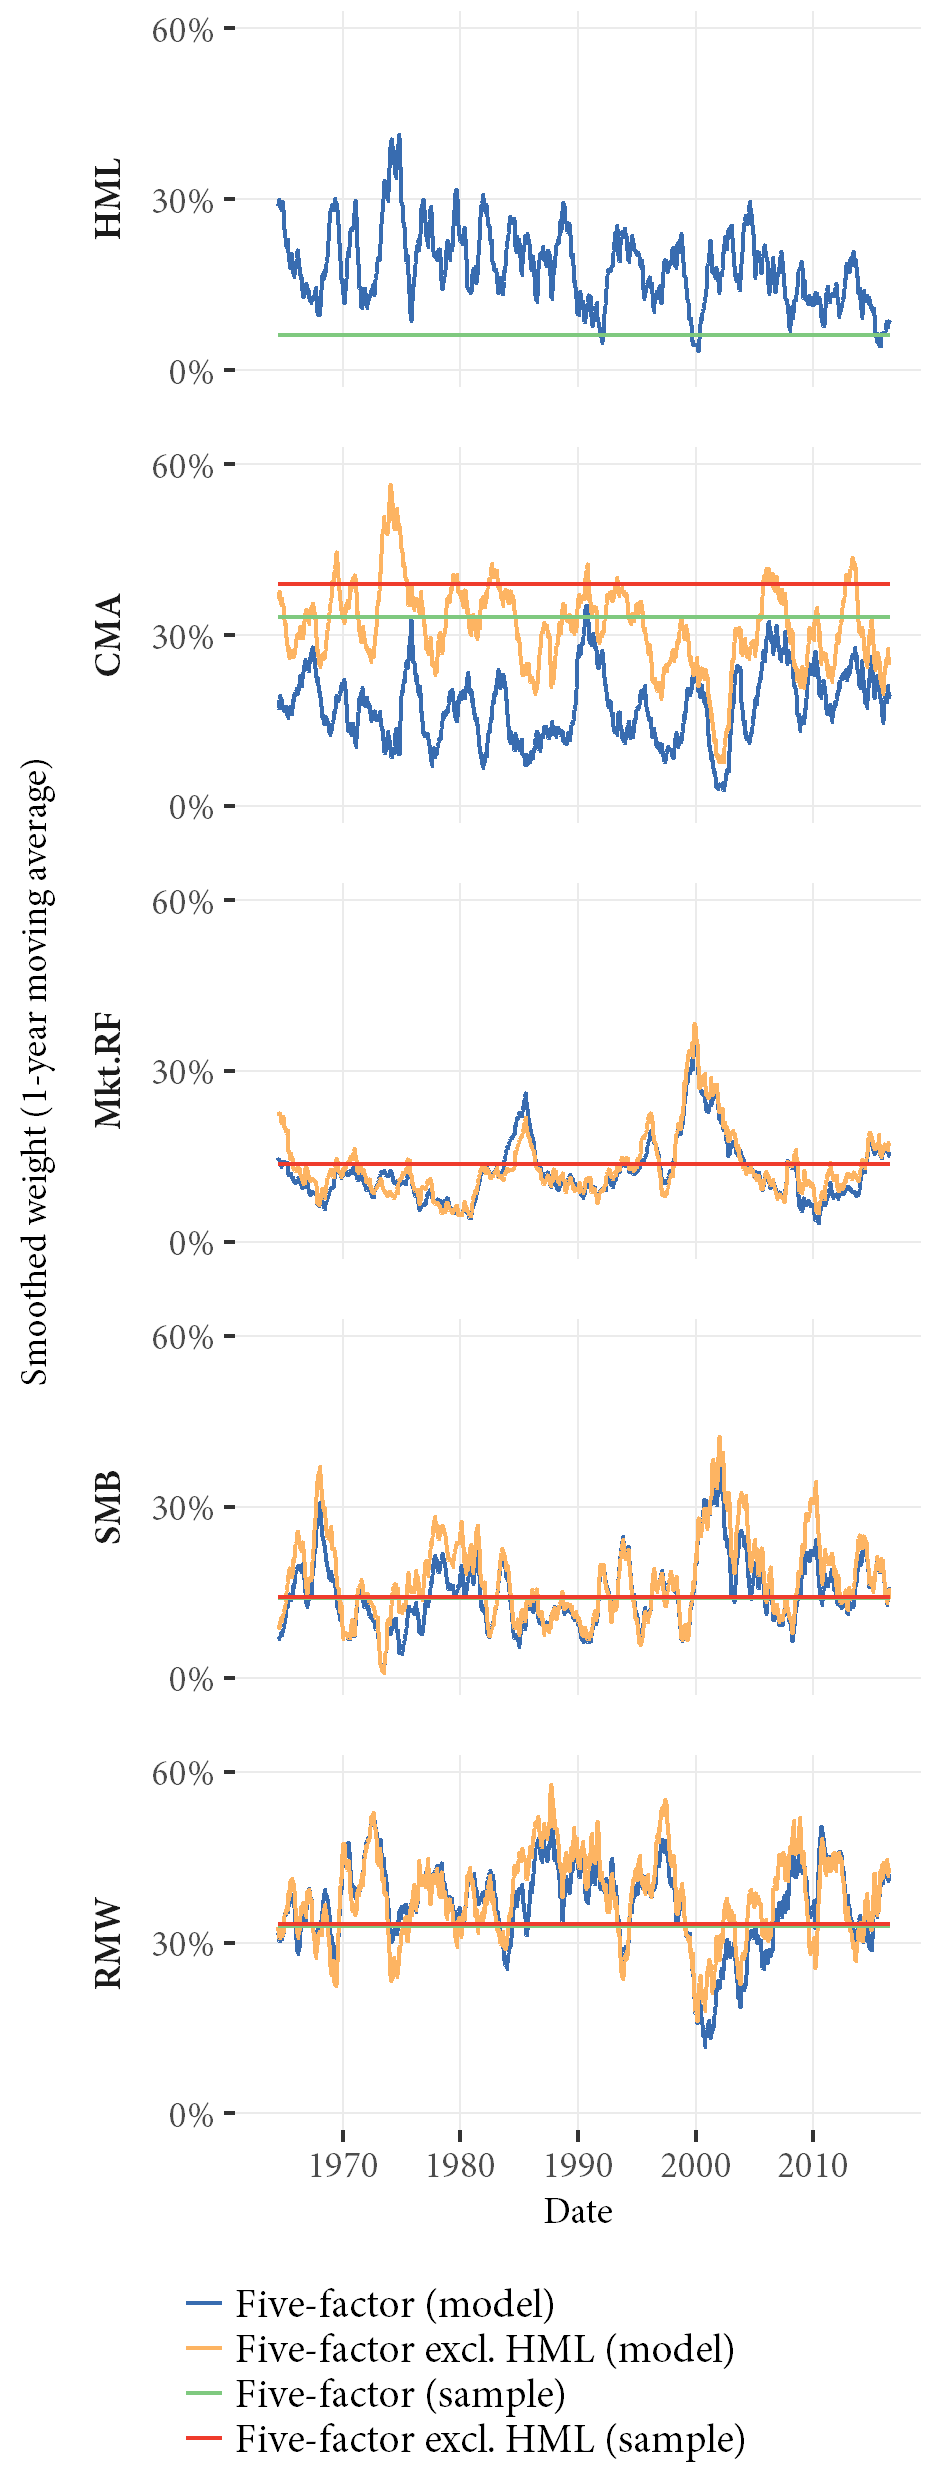
\includegraphics[scale = 1]{graphics/Weights_5F_EXCL_HML_5F.png}
  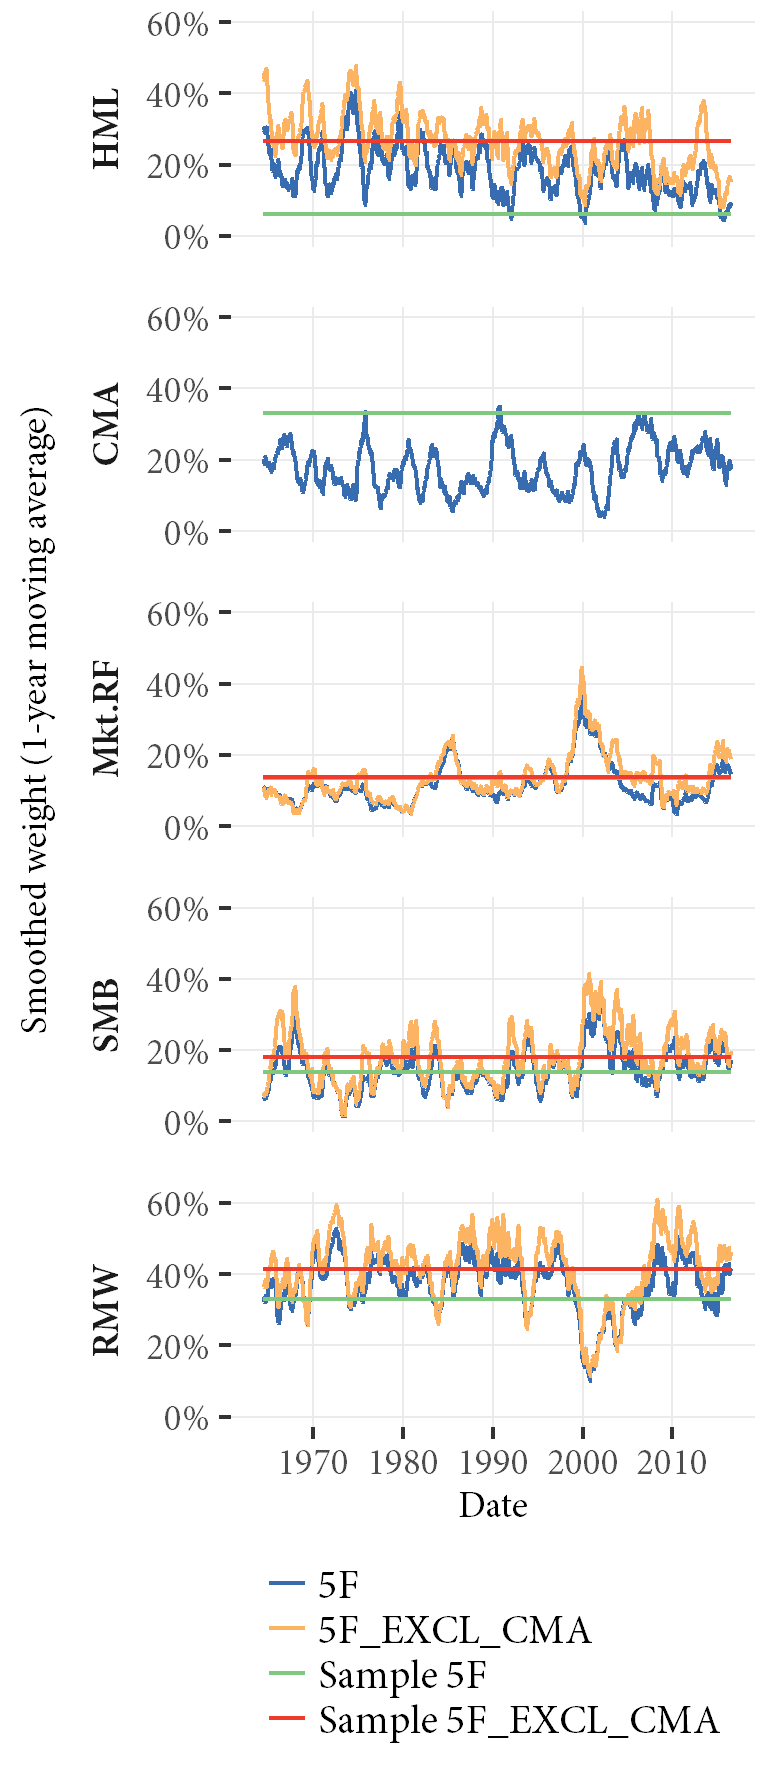
\includegraphics[scale = 1]{graphics/Weights_5F_EXCL_CMA_5F.png}
\end{figure}

We begin by examining the left column of plots in \autoref{fig:mv_optimal_5} that includes and excludes HML. First, we note that the weight of HML is not zero when introduced in the investible universe. This appears to be the case for both the sample estimate of means and covariances, as well as the dynamic estimates from the copula model. Both inputs suggest that HML does in fact improve the tangency portfolio, as the optimal portfolio has a positive weight on the factor. 

Although we impose the additional restriction of no negative weights, this finding does stand in contrast to the conjecture in \textcite{FF2015} that HML should not improve the tangency portfolio. While the unconstrained tangency portfolio may or may not include HML, the simple restriction of no negative weights makes HML an important part of the optimal portfolio. We notice that the sample inputs result in a lower allocation to HML in the full five-factor-model, of approx. 6\%, while the average weight under dynamic weights is 18\%. A table of average weights under the different asset universes is given in \autoref{tab:mv_realized_insample_5F}.

Second, we note that the dynamic weight of HML seems to be highly similar to the decrease in weight in CMA, while all the remaining factors seem to stay very close to their original weights when moving to the six-factor model. In other words, the weight that is attributed to HML is drawn nearly directly from the weight of CMA, in each period. Our interpretation is that in a five-factor excluding HML, CMA proxies for HML, which is why CMA absorbs nearly all the weight. HML also seems to proxy for CMA to a lesser extent, as shown by the right hand column of plots, which include and exclude CMA. When CMA is included, the weight of HML is significantly lowered, but so are the weights of SMB and RMW. The proxying behavior of HML and CMA is expected, as the factors are highly correlated and zero-cost portfolio regressions in this thesis (\autoref{fig:abnormal}), as well as in \textcite{FF2015} and \textcite{Asness2015}, indicate that the main explanatory variable for HML is CMA, and vice versa.

The above results are similar when we repeat the mean-variance optimizations in the six-factor-model universe excluding HML and CMA, see \autoref{fig:mv_optimal_6} and \autoref{tab:mv_realized_insample_6F}. Using both sample inputs and copula inputs, we find no reason to believe that mean-variance investing in the HML factor is dead or fully subsumed by the remaining factors.

\begin{figure}[htbp]
  \centering
  \footnotesize
  \renewcommand{\arraystretch}{1.2}
  \caption{Mean-variance optimal weights in the six-factor universe \\ \quad \\ Smoothed as 1-year moving averages. Left hand panel including and excluding HML, right hand including and excluding CMA. Based on one-week-ahead forecasts from the copula model 1963--2016.}
  \label{fig:mv_optimal_6}
  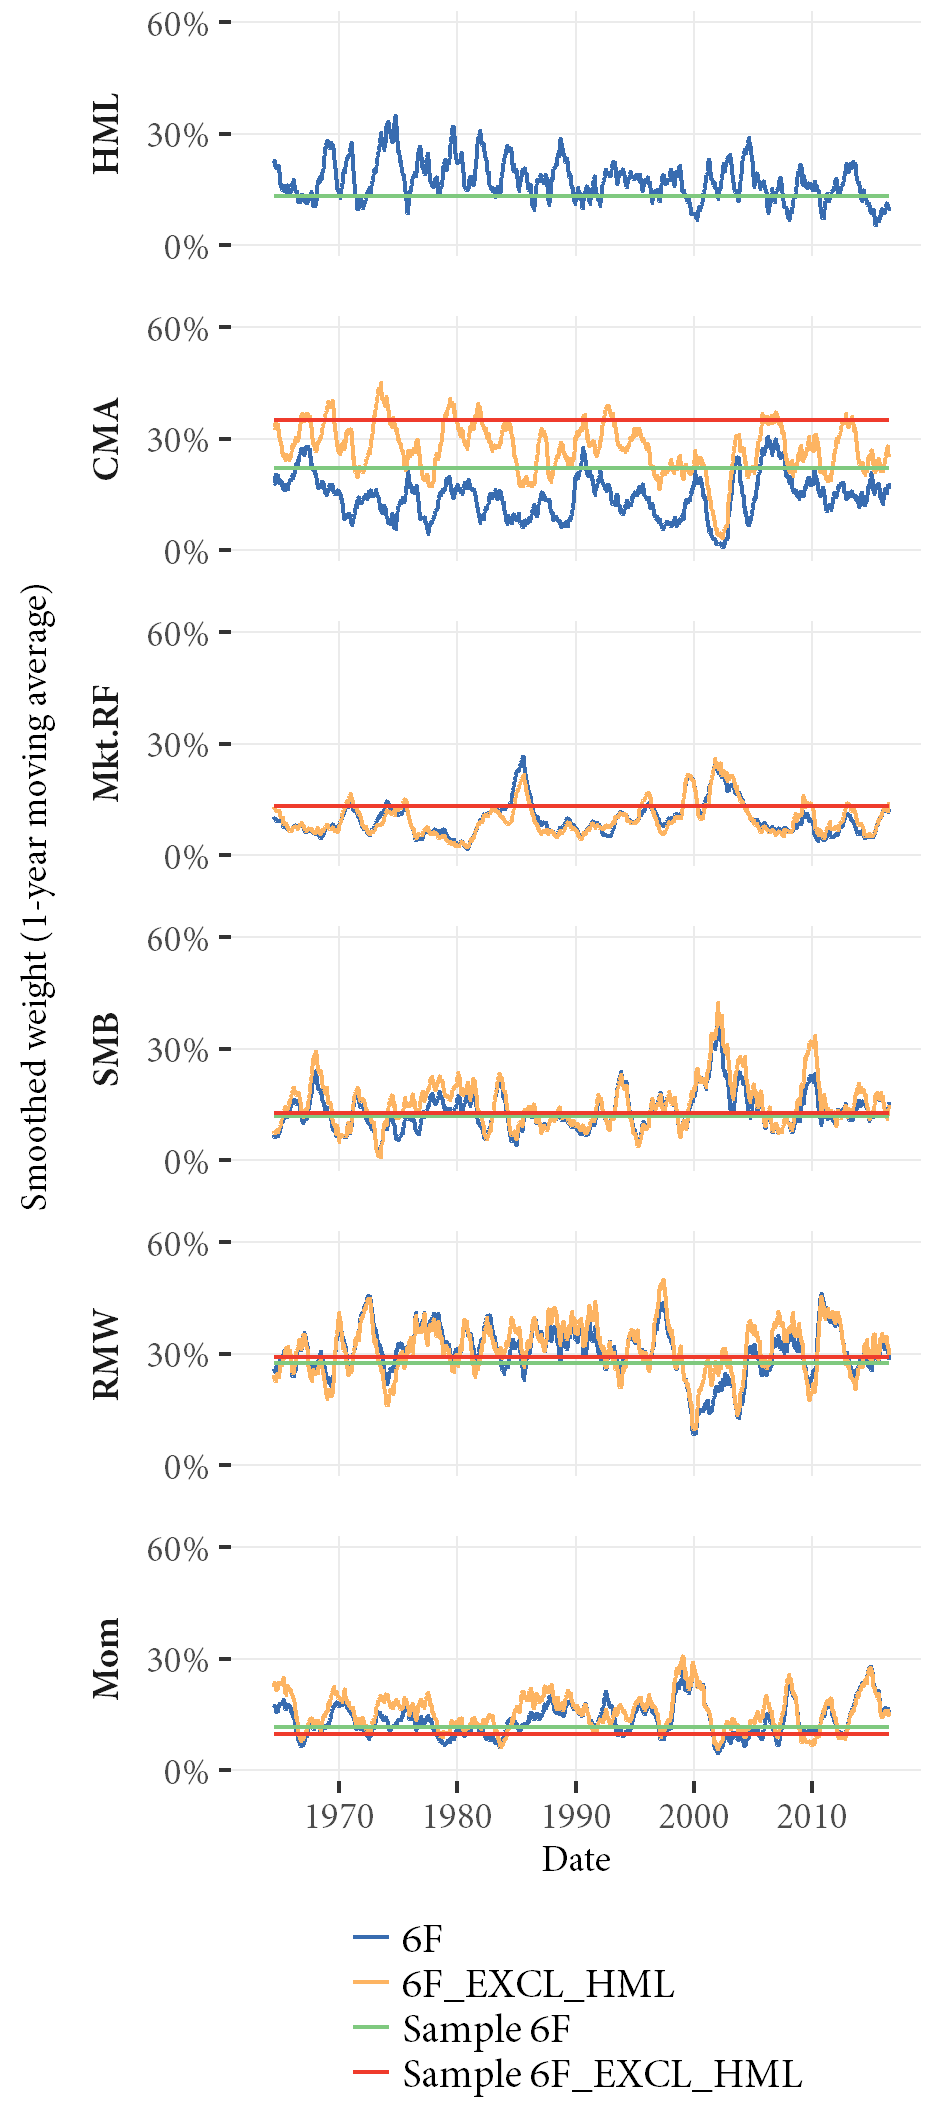
\includegraphics[scale = 1]{graphics/Weights_6F_EXCL_HML_6F.png}
  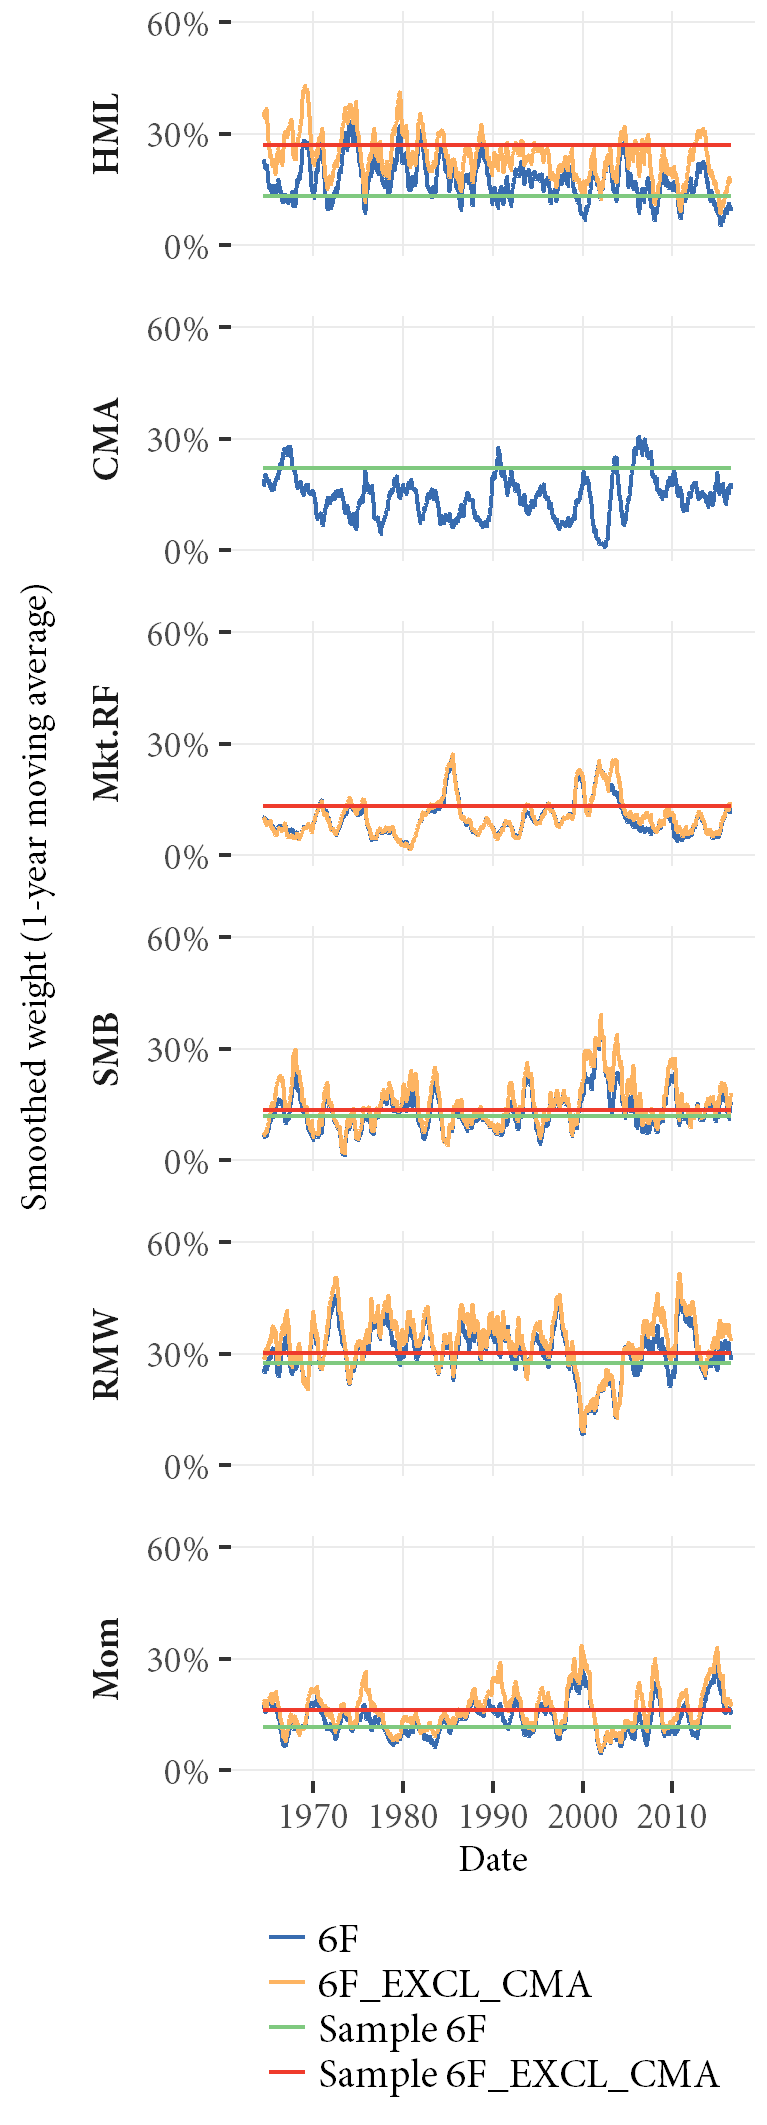
\includegraphics[scale = 1]{graphics/Weights_6F_EXCL_CMA_6F.png}
\end{figure}

\begin{table}
  \centering
  \footnotesize
  \renewcommand{\arraystretch}{1.2}
  \caption{Average portfolio weights: Five-factor model \\ \quad \\ Based on sample inputs as well as dynamic copula model inputs, in-sample (1963--2016). All weights expressed in percentages.}
  \label{tab:mv_realized_insample_5F}
  \begin{tabularx}{\textwidth}{@{\extracolsep{5pt}} X ddd d ddd @{}}
    \toprule

    & 
      \multicolumn{7}{c}{Five-factor model} \\
      \cmidrule{2-8}
    &
      \multicolumn{3}{c}{Model} &&
      \multicolumn{3}{c}{Sample} \\
    \cmidrule{2-4} \cmidrule{6-8}

    &
      \multicolumn{1}{c}{All} &
      \multicolumn{1}{c}{excl. CMA} &
      \multicolumn{1}{c}{excl. HML} &&
      \multicolumn{1}{c}{All} &
      \multicolumn{1}{c}{excl. CMA} &
      \multicolumn{1}{c}{excl. HML} \\
    \midrule
    \textbf{Average weights} \\
    Mkt.RF & 12.4 & 14.2 & 13.2 && 13.6 & 13.8 & 13.7 \\
    SMB    & 15.0 & 18.3 & 17.4 && 14.0 & 18.0 & 14.1 \\
    HML    & 18.2 & 26.3 &        && 6.2  & 26.7 &       \\
    CMA    & 17.6 &        & 31.4 && 33.2 &        & 39.0 \\
    RMW    & 36.8 & 41.2 & 38.0 && 33.0 & 41.5 & 33.2 \\
    \midrule
    \textbf{Difference to full five-factor model} \\
    Mkt.RF & &   1.8 &   0.8 && &   0.2 &   0.1 \\
    SMB    & &   3.3 &   2.4 && &   4.0 &   0.1 \\
    HML    & &   8.1 & -18.2 && &  20.5 &  -6.2 \\
    CMA    & & -17.6 &  13.8 && & -33.2 &   5.8 \\
    RMW    & &   4.4 &   1.2 && &   8.5 &   0.2 \\
    \cmidrule{3-4} \cmidrule {7-8}
    \textbf{Sum} & & 0.0 & 0.0 &&  & 0.0 & 0.0 \\
     \bottomrule
  \end{tabularx}
\end{table}

\begin{table}
  \centering
  \footnotesize
  \renewcommand{\arraystretch}{1.2}
  \caption{Average portfolio weights: Six-factor model \\ \quad \\ Based on sample inputs as well as dynamic copula model inputs, in-sample (1963--2016). All weights expressed in percentages.}
  \label{tab:mv_realized_insample_6F}
  \begin{tabularx}{\textwidth}{@{\extracolsep{5pt}} X ddd d ddd @{}}
    \toprule

    & 
      \multicolumn{7}{c}{Six-factor model} \\
      \cmidrule{2-8}
    &
      \multicolumn{3}{c}{Model} &&
      \multicolumn{3}{c}{Sample} \\
    \cmidrule{2-4} \cmidrule{6-8}

    &
      \multicolumn{1}{c}{All} &
      \multicolumn{1}{c}{excl. CMA} &
      \multicolumn{1}{c}{excl. HML} &&
      \multicolumn{1}{c}{All} &
      \multicolumn{1}{c}{excl. CMA} &
      \multicolumn{1}{c}{excl. HML} \\
    \midrule
    \textbf{Average weights} \\
    Mkt.RF & 9.8  & 10.4  & 9.9  && 13.2 & 13.2 & 13.4 \\
    SMB    & 13.4 & 15.6 & 15.3 && 12.0 & 13.4 & 12.7 \\
    Mom    & 13.9 & 16.6 & 15.9 && 11.7 & 16.2 & 9.7  \\
    HML    & 17.6 & 24.1 &        && 13.2 & 27.0 &        \\
    CMA    & 14.6 &        & 27.5 && 22.2 &        & 35.2 \\
    RMW    & 30.6 & 33.3 & 31.4 && 27.7 & 30.2 & 29.0 \\
    \midrule
    \textbf{Difference to full six-factor model} \\
    Mkt.RF & &   0.6 &   0.1 && &   0.0 &   0.2 \\
    SMB    & &   2.2 &   1.9 && &   1.4 &   0.7 \\
    Mom    & &   2.7 &   2.0 && &   4.5 &  -2.0 \\
    HML    & &   6.5 & -17.6 && &  13.8 & -13.2 \\
    CMA    & & -14.6 &  12.9 && & -22.2 &  13.0 \\
    RMW    & &   2.7 &   0.8 && &   2.5 &   1.3 \\
    \cmidrule{3-4} \cmidrule {7-8}
    \textbf{Sum} & & 0.0 & 0.0 &&  & 0.0 & 0.0 \\
    \bottomrule
  \end{tabularx}
\end{table}

